% TODO list:
% - Add sage and magma to refs.
% - Include thanks? anyone else?
% - How will code be included, snippets or on disk??
% - Think about typography
% - Proofs/detailed arguments for correctness of algos.
% - Add input output to algos

% Structure:
% - Introduction
% - Background
% - Problem
% -  History??
% -- Statements
% -- Quadratics
% -- Cubics?
% -- Cocyclics
% -- Monogenics
% -- General absolute
% -- General relatives
% - Applications to elliptics over Q
% - Conclusion

% Include project managementy bits
% Practical considerations, lines of code, sage vs magma python etc.

\documentclass[12pt,a4paper,abstracton,bibtotoc]{scrreprt}

\author{Alex J. Best \\ Supervised by Dr. Lassina Demb\'el\'e}
\date{2014}
\title{Finding orders with prescribed index in number fields}

\usepackage{amsmath, amssymb, amsfonts, amsthm, hyperref, listings, tikz, algorithm2e, graphicx, enumerate}
\usepackage[utf8]{inputenc}
\usepackage[T1]{fontenc}
\usepackage[english]{babel}
\usepackage{setspace}
\onehalfspacing

\theoremstyle{definition}
\newtheorem{thm}{Theorem}
\newtheorem{lem}{Lemma}
\newtheorem{cor}{Corollary}
\newtheorem{prop}{Proposition}
\newtheorem{defn}{Definition}
\newtheorem{defns}{Definitions}
\newtheorem{prob}{Problem}
\newtheorem{ex}{Example}
\newtheorem{rem}{Remark}
\newtheorem{nota}{Notation}
\newtheorem{alg}{Algorithm}

\setcounter{tocdepth}{3}

\lstset{
basicstyle=\footnotesize,       % the size of the fonts that are used for the code
showspaces=false,               % show spaces adding particular underscores
showstringspaces=false,         % underline spaces within strings
showtabs=false,                 % show tabs within strings adding particular underscores
frame=single,           % adds a frame around the code
captionpos=b,           % sets the caption-position to bottom
breaklines=true,        % sets automatic line breaking
breakatwhitespace=false,    % sets if automatic breaks should only happen at whitespace
}

\graphicspath{{img/}}

\newcommand{\QQ}{\mathbf{Q}}
\newcommand{\RR}{\mathbf{R}}
\newcommand{\CC}{\mathbf{C}}
\newcommand{\ZZ}{\mathbf{Z}}
\newcommand{\p}{\mathfrak{p}}
\renewcommand{\O}{\mathcal{O}}

\DeclareMathOperator{\Orders}{Orders}
\DeclareMathOperator{\Ann}{Ann}
\DeclareMathOperator{\End}{End}
\DeclareMathOperator{\Mat}{Mat}
\DeclareMathOperator{\im}{im}

\begin{document}
\maketitle

\begin{abstract}
%TODO insert very small backstory, orders are objects in ant here ..
Orders in number fields are common objects of study in algebraic number theory.
Here we develop methods to obtain all orders with a specified index inside another given one.
The performance, both theoretically and in implementations of these methods is discussed.
We also apply these techniques to problems relating to elliptic curves over the rational numbers.

\smallskip
\noindent \textbf{Keywords.} Number theory, algebraic number theory, elliptic curves, number fields, algorithms.
\end{abstract}

\tableofcontents

\chapter{Introduction}
In this report we develop algorithmic methods for the solution of a problem arising from algebraic number theory. 
We detail some interesting situations in which this algorithm can be applied at the end.

The report is organised as follows.
We first go through the background material needed to motivate, define and describe the solution of our problems in chapter~\ref{chap:background}.
In section~\ref{sec:ca} we cover some commutative algebra dealing with the basic properties of modules over rings, after this in section~\ref{sec:ant} we move into algebraic number theory defining the key notions needed to study orders and considering the reasons such ideas were introduced.
We finish up the background material in section~\ref{sec:ell} with an introduction to the theory of elliptic curves, which will be one of the interesting areas we will apply our methods to.

Chapter~\ref{chap:prob} is where we consider our main problem and solutions to it.
In section~\ref{sec:statements} we define the problems themselves and discuss the interest in studying them.
After this in the rest of chapter~\ref{chap:prob} we detail the techniques used to solve the problems considered, starting with some special cases before moving onto more general results.
Next we discuss the advantages of the algorithms developed and their practial timings.

Finally in section~\ref{sec:ellapp} we move on to some interesting applications of these methods to the study of elliptic curves.


\chapter{Background material}
\label{chap:background}

In this section we fix several definitions and important results from algebraic number theory and commutative algebra.
We assume only fairly basic knowledge of abstract algebra, such as the notions of groups, rings and fields.

The results given here are well known and are used throughout the rest of the report.

\section{Commutative algebra}
\label{sec:ca}
We introduce several notions and results that will be useful to us throughout the report, proofs for those results not proved here can be found in many textbooks on commutative algebra, such as \cite{am} or \cite{matsumura}.

All rings here are commutative with an identity element.
\begin{defn}[Module]
Given a ring $R$ we define an \emph{$R$-module} $M$ to be an abelian group under addition, with a scalar multiplication map $\cdot \colon R\times M \to M$ satisfying
\begin{align*}
1\cdot m &= m \; &&\text{for all } m\in M \\
r_1\cdot(r_2 \cdot m) &= (r_1r_2)\cdot m \; &&\text{for all } r_1,r_2\in R,\; m\in M \\
r\cdot(m_1 + m_2) &= r\cdot m_1 + r\cdot m_2 \; &&\text{for all } r\in R, \; m_1,m_2\in M \\
(r_1 + r_2)\cdot m &= r_1\cdot m + r_2\cdot m \; &&\text{for all } r_1,r_2\in R, \; m_1\in M
\end{align*}
\end{defn}

We often refer to elements of the ring $R$ as \emph{scalars}.

From now on we will omit the notation $\cdot$ for scalar multiplication as it will be clear from context when the multiplication is taking place in the ring $R$ or on a module $M$.
We will also not make explicit the ring $R$ involved if it is not relevant to the discussion at hand, instead referring simply to a \emph{module}.

The most common modules we will use here will be $\ZZ$-modules such as:
\begin{ex}
\[
\ZZ,\ \{(a,b)\mid a,b\in \ZZ\},\text{ or }\{a\sqrt{2} + b\sqrt[3]{2}\mid a,b\in \ZZ\}.
\]
\end{ex}
In fact every abelian group can be given a $\ZZ$-module structure so of course they are ubiquitous in commutative algebra, nevertheless it is useful to think of the modules used here in terms of $\ZZ$ rather than as abstract abelian groups.
We now list some standard definitions that are used to talk about how different modules relate to one another and describe ways of constructing new modules from old.

\begin{defn}[Module homomorphism]
Given $R$-modules $M_1$ and $M_2$, a function $f\colon M_1 \to M_2$ satisfying
\begin{align*}
f(rm) &= rf(m) &&\text{ for all $r\in R$, $m\in M_1$}\\
f(m + m') &= f(m) + f(m')&&\text{ for all $m,m'\in M_1$}
\end{align*}
is called an \emph{$R$-module homomorphism} or simply a \emph{module homomorphism} when the ring is clear.
We also use the term map for this concept.
\end{defn}

\begin{defn}[Isomorphism of modules]
Two $R$-modules $M_1$ and $M_2$ are said to be \emph{isomorphic} is there exists a bijective module homomorphism between them. 
In this case we write $M_1\cong M_2$.
\end{defn}

Module isomorphism is an equivalence relation on the class of all modules and so we often think of two isomorphic modules as being the same, just written in a different manner.

\begin{defn}[Submodule]
A \emph{submodule} $N$ of a module $M$ is a module whose elements all belong to $M$ and whose operations are the same as those from $M$ on the elements on $N$.
\end{defn}

\begin{defn}[Quotient module]
The \emph{quotient module} of two $R$-modules $M$ and $N$ with $M$ a submodule of $N$ is defined to be the quotient abelian group under addition $N/
M$ with scalar multiplication given by
\[
r\cdot(m + N) = rm + N\text{ for all $r\in R$, $m\in M$}.
\]
\end{defn}

\begin{defn}[Index]
Given a module $M$ that is a submodule of a module $N$ the \emph{index} of $M$ in $N$, denoted $[N:M]$ is the size of the quotient module $N / M$.
\end{defn}

\begin{defn}[Direct sum]
Given two $R$-modules $M_1$ and $M_2$ we define their \emph{direct sum} (denoted $\oplus$) to be the module with element set $M_1 \times M_2$ and operations given by the operations of $M_1$ and $M_2$ performed elementwise. i.e.
\begin{align*}
r\cdot(m_1,m_2) &= (r\cdot m_1, r\cdot m_2)\\
(m_1,m_2) + (m_1',m_2') &= (m_1 + m_1',m_2+m_2').
\end{align*}
\end{defn}

Not that this is in general distinct from when we have $M_1$ and $M_2$ submodules of some module $N$ and write
\[
M_1 + M_2 = \{m_1 + m_2 \mid m_1\in M_1,\ m_2\in M_2\}.
\]
For example with this elementwise addition we have $M + M = M$ for any module $M$, whereas $M\oplus M$ is not isomorphic to $M$ unless $M$ is the trivial module (i.e. the module containing only a zero element and no others).

The well known isomorphism theorems also hold for modules, we require only two.

\begin{thm}[First isomorphism theorem for modules]
Given a surjective module homomorphism $f\colon M \to N$ the kernel of $f$ is a submodule of $M$ and
\[
M/\ker(f) \cong N.
\]
\end{thm}

\begin{thm}[Third isomorphism theorem for modules]
Given a chain of submodules $M_1 \subseteq M_2 \subseteq M_3$ the quotient module $M_2/M_1$ is a submodule of $M_3/M_1$ and we have an isomorphism
\[
(M_3/M_1)/(M_2/M_1) \cong (M_3/M_2).
\]
\end{thm}

An easy consequence of this relating the indices of submodules is worth noting.

\begin{cor}
\label{cor:indexmult}
Given a chain of submodules $M_1 \subseteq M_2 \subseteq M_3$ we have
\[
[M_3:M_1] = [M_3:M_2][M_2:M_1].
\]
\end{cor}

\minisec{}
We now define a property of modules that makes them easier to work with and, importantly, easier to do computations with.

\begin{defn}[Finitely generated]
An $R$-module $M$ is \emph{finitely} generated if there is a \emph{finite} set $B\subset M$ such that any $m\in M$ can be written as
\[m = \sum_{b\in B} \alpha_b b\]
for some coefficients $\alpha_b \in R$.
\end{defn}

\begin{defn}[Torsion submodule]
The \emph{torsion submodule} $M_\text{tors}$ of an $R$-module $M$ is the set
\[
\{m\in M \mid \exists\; r \in R\setminus 0 \text{ such that } rm = 0\}.
\]
This is the set of elements that are killed by some non-zero scalar.
As implied by the name this is always submodule of $M$.
\end{defn}

A module $M$ is called a torsion module if $M_\text{tors} = M$, and torsion-free if $M_\text{tors} = 0$.

% TODO generalise to module over PID

\begin{defn}[Rank of a $\ZZ$-module]
Given a $\ZZ$-module $M$ we can always write $M = M_\text{tors} \oplus \ZZ^r$ for some unique $r\in \ZZ_{\ge 0}$.
This $r$ is called the \emph{rank} of the $\ZZ$-module.
\end{defn}

\begin{ex}
\[M = \ZZ^2 = \{(a,b)\mid a,b\in \ZZ\}\]
is a torsion free $\ZZ$ module. Let
\[N = \{(2c,0) \mid c\in\ZZ\} \cong \ZZ\]
be a submodule of $M$.
Then the quotient module
\[M/N \cong (\ZZ/2\ZZ)\times \ZZ\]
has torsion submodule $(M/N)_\text{tors}$ equal to $\ZZ/2\ZZ$ and is of rank 1.
\end{ex}

\begin{defn}[Short exact sequence]
A \emph{short exact sequence of $R$-modules} is a sequence of $R$-modules and maps between them, drawn as
\[
0 \to M_1 \xrightarrow{f_1} M_2 \xrightarrow{f_2} M_3 \to 0
\]
such that for every occurrence of a triple $N_1 \xrightarrow{g_1} N_2 \xrightarrow{g_2} N_3$ we have $\im(g_1) = \ker(g_2)$.
\end{defn}

In any short exact sequence we therefore have $f_1$ injective and $f_2$ surjective.

\begin{defn}[Split short exact sequence]
A short exact sequence $0 \to M_1 \xrightarrow{q} M_2 \xrightarrow{r} M_3 \to 0$ is called \emph{split} if any of the following equivalent conditions hold:
\begin{enumerate}[(i)]
\item There is a map $t\colon M_2 \to M_1$ such that $t\circ q$ is the identity on $M_1$.
\item There is a map $u\colon M_3 \to M_2$ such that $u\circ r$ is the identity on $M_2$.
\item $M_2 \cong M_1 \oplus M_3$.
\end{enumerate}
\end{defn}


\section{Algebraic number theory}
\label{sec:ant}

Algebraic number began with the study of algebraic numbers and their uses in solving Diophantine equations.
The subject has since expanded to encompass a huge amount of mathematics involving the use of algebraic techniques to tackle number theoretic problems. %TODO ????
As above, more details about anything not proved here can be found in any of the many texts on algebraic number theory, for example \cite{neukirch}, \cite{lang}, \cite{narkiewicz} or \cite{stewtall}.

\begin{defn}[Number field]
A \emph{number field} $K$ is a field that is also a finite dimensional $\QQ$-vector space.
\end{defn}

\begin{ex}\label{ex:quad}
We write $\QQ(\sqrt{3})$ for the smallest field containing both $\QQ$ and $\sqrt{3}$, it is clear that the set
\[
\{a + b\sqrt{3}\mid a,b \in \QQ\}
\]
must be contained in such a field.
But we can also see that this set is closed under addition, subtraction, multiplication and non-zero division, and hence this set is the field $\QQ(\sqrt{3})$.

Here we see that $\QQ(\sqrt{3})$ has dimension 2 as a vector space over $\QQ$.
\end{ex}

\begin{defn}[Degree of a number field]
The dimension of a number field $K$ as a $\QQ$ vector space is called the \emph{degree} of $K$, denoted $[K:\QQ]$.

We say that number fields of degree 2, such as in example~\ref{ex:quad} above are \emph{quadratic}.
Similarly degree 3 number fields are called \emph{cubic}.
\end{defn}

\minisec{}
The following few definitions are central to the whole problem.

A number field will have a large quantity of subrings, only some of which are of real number theoretic interest.
So we distinguish some subrings that have desirable properties and single them out for study.

\begin{defn}[Order]
An \emph{order} of a number field $K$ is a subring of $K$ that is finitely generated as a $\ZZ$-module, and of rank equal to the degree of $K$ (this is the maximal rank).
\end{defn}

By definition orders have finite bases over $\ZZ$ and so we will often represent orders by writing them as sums 
\[
\O = \ZZ\alpha_1 + \ZZ \alpha_2 + \cdots + \ZZ \alpha_n.
\]
We also use the notation $\ZZ[\alpha]$ to mean the ring of polynomials expressions in $\alpha$ with integer coefficients, provided $\alpha$ is an algebraic integer this will be an order.

\begin{defn}[Ring of integers]
The \emph{ring of integers}, denoted $\ZZ_K$, of a number field $K$ is the unique maximal order.
\end{defn}

The terminology for this ring comes from the fact that its behaviour is analogous to the way $\ZZ$ behaves inside $\QQ$.
As we will see later the maximal order of a quadratic number field is easy to determine but the complexity of such calculations increases with the degree.

The notion of index introduced earlier applies here and as all orders lie inside the ring of integers we can always find the index of an order $\O$ inside $\ZZ_K$.
If we just use the term index of an order, without specifying another containing it, we will mean exactly this, the index inside the maximal order.

\begin{ex}
\[
[\ZZ\cdot 1 + \ZZ\cdot \sqrt{2} : \ZZ \cdot 1 + \ZZ \cdot 2\sqrt{2}] = 2.
\]
\end{ex}

In figure~\ref{fig:sageord} one embedding into the complex plane of the ring of integers of $\QQ[x]/(x^2 + 19)\cong \QQ(\sqrt{-19})$ is shown.
Highlighted in bold is a suborder of index 3 in this order.
\begin{figure}
\centering
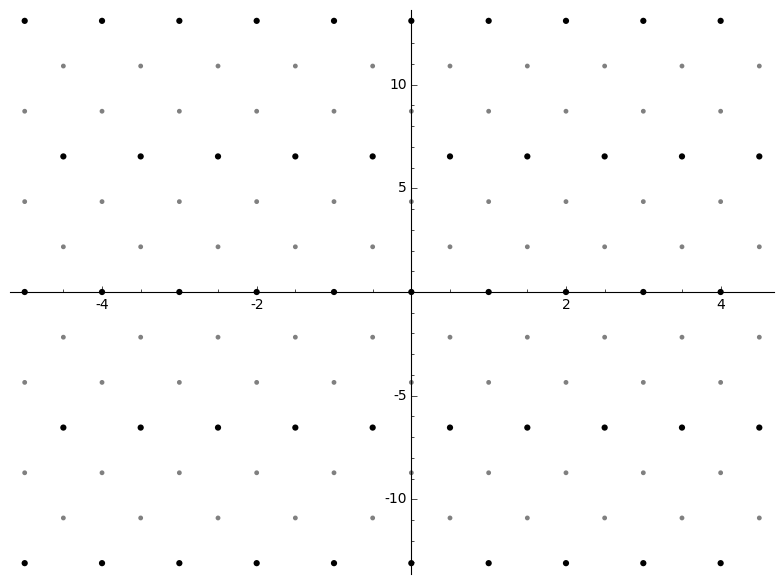
\includegraphics[scale=0.6]{sageord}
\caption{\label{fig:sageord} An embedding in $\CC$ of the ring of integers of $\QQ(\sqrt{-19})$ and an index 3 suborder.}
\end{figure}

%P.<x> = QQ[]
%K = NumberField(x^2 + 19, 'a')
%ZK = K.maximal_order()
%OK = K.order(3*ZK.0)
%print ZK.basis()
%f = K.embeddings(CC)[0]
%pts = []
%pts2 = []
%for x in range(-10,10):
%    for y in range(-10,10):
%        if f(x*ZK.0 + y*ZK.1).imag().abs() < 15: 
%            pts.append(f(x*ZK.0 + y*ZK.1))
%        if f(x*OK.0 + y*OK.1).imag().abs() < 15: 
%            pts2.append(f(x*OK.0 + y*OK.1))
%
%list_plot(pts,color="gray",size=12) + list_plot(pts2,color="black",size=20)


\section{Elliptic curves}
\label{sec:ell}

We now introduce the background material relevant to elliptic curves, one of the intended applications of these methods.
This is not required for the main problem discussed in chapter~\ref{chap:prob}, but section~\ref{sec:ellapp} uses these ideas heavily.
As with the above sections everything here can be found in textbooks on elliptic curves (such as \cite{knapp} or \cite{cassels}), we offer a rapid summary, moving quickly to the notions relevant to the project in this overview.

\begin{defn}[Elliptic curve]
For us an \emph{elliptic curve} $E$ defined over a field $K$ will be given by a binary cubic equation of the form
\[
y^2 + a_1xy + a_3y = x^3 + a_2x^2 + a_4x + a_6\text{ with }a_i\in K.
\]
To such a curve we assign several $b$ invariants based on the coefficients in the definition as follows
\begin{align*}
b_2 &= a_1^2 + 4a_2\\
b_4 &= 2a_4 + a_1a_3\\
b_6 &= a_3^2 + 4a_6\\
b_8 &= a_1^2a_6 + 4a_2a_6 - a_1a_3a_4 + a_2a_3^2 -a_4^2.
\end{align*}
We then also require that the \emph{discriminant} $\Delta$ of $E$, given by
\[
\Delta = -b_2^2b_8 -8b_4^3 -27b_6^2 +9b_2b_4b_6
\]
is not zero for $E$ to really be an elliptic curve.

Given an elliptic curve $E$ defined over a field $K \subset K'$ another field, we let $E(K')$ be the set of points in $K'\times K'$ satisfying the equation defining $E$, along with an extra point $\infty$.
This additional point is called the point at infinity, the reasons for its inclusion in the set should become clear later.
\end{defn}

The condition on $\Delta$ given above is to ensure that our curve does not have any points where both the derivatives with respect to $x$ and $y$ vanish, such a point is called a singular point and the existence of such a point causes the behaviour of the curve to differ highly from what we would normally expect.

\begin{ex}
Let 
\[
E \colon y^2 + 2xy + y = x^3 - 2x + 3
\]
be an elliptic curve.
Then we can see that $(1,(\sqrt{17}-3)/2)\in E(\RR) \subset E(\CC)$ as the coordinates satisfy the equation defining the curve.

We can plot the real points of this curve, such a plot is shown in figure~\ref{fig:ec}.
This plot of the real points is typical for an elliptic curve, though there can easily be two connected components rather than one as in this case.
\begin{figure}
\centering
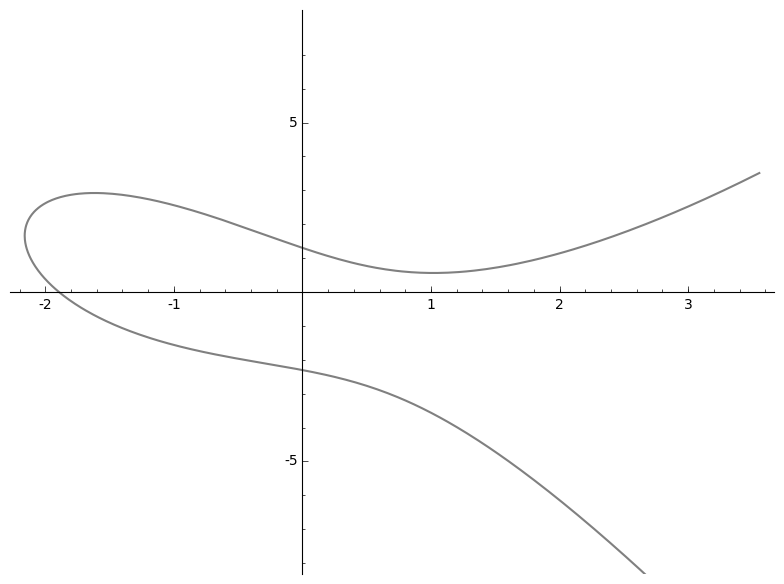
\includegraphics[scale=0.6]{sageec}
\caption{\label{fig:ec}The real points of $E \colon y^2 + 2xy + y = x^3 - 2x + 3$.}
\end{figure}
\end{ex}

One of the things that makes elliptic curves so interesting to study is the fact that we can define a natural way of adding points of the curve over some field, with this definition the set of points on the curve becomes a group.

\begin{defn}[Group law]
We define the sum of two points $P,Q\in E(K)$ as follows, let $L$ be the line joining $P$ and $Q$ (take $L$ to be the tangent at $P$ if $P=Q$).
Then $L$ intersects $E$ in three points (with multiplicity) so there is one point in addition to $P$ and $Q$ on both $L$ and $E$, call this point $R$.
Now there is at most one other point with the same $x$ coordinate as $R$ that lies on $E$, this is our sum $P+Q$.
\end{defn}

With this definition of addition the set of points of $E$ over some field $K$ is a group, and moreover this group is abelian (as the line through $P$ and $Q$ is the same as the line through $Q$ and $P$).
From now on we will denote the point $\infty\in E(K)$ as $0$, but still refer to it as \emph{at infinity}.

As remarked above any abelian group can be regarded as a $\ZZ$-module $M$ in a natural way by letting 
\[n\cdot z = \underbrace{z + z + \cdots + z}_\text{$n$ times},\text{ for } n\in\ZZ_{\ge 0},\ z\in M\]
and letting $n\cdot z = (-n)\cdot(-z)$ for negative $n\in \ZZ$.
With this idea in mind $E(K)_\text{tors}$ is the set of points of $E$ defined over $K$ that can be added to themselves some finite number of times to get the point at infinity.
This is often called the \emph{torsion subgroup} of $E$.
It turns out that when $K = \QQ$ there are only a finite number of groups that $E(\QQ)_\text{tors}$ can be.

\begin{thm}[Mazur's torsion theorem]
\label{thm:tors}
Given an elliptic curve $E$ defined over the rationals $E(\QQ)_\text{tors}$ is one of:
\[
\ZZ/i\ZZ,\text{ for } i \in\{1,2,\ldots,9,10,12\}\text{ or }
\ZZ/2\ZZ \times \ZZ/2i\ZZ,\text{ for } i \in\{1,2,3,4\}.
\]
\end{thm}

In fact similar results have been obtained for quadratic fields too, for more detail on what is known about the torsion subgroup of an elliptic curve over a number field see \cite{sutherland}.

Sometimes it is necessary to talk about smaller subgroups of this group whose elements have order dividing some fixed $n$ and so we introduce the following definition.
\begin{defn}[$n$-division points]
For some $n\in\ZZ$ the set of \emph{$n$-division points} of $E$ over $K$ is
\[
E(K)[n] = \{P\in E(K) \mid nP = 0\}.
\]
\end{defn}
Although $E(\QQ)_\text{tors}$ cannot be large by theorem~\ref{thm:tors} it is still useful to consider the $n$-division points of a curve over the rationals and we will use this group later.

\minisec{}
We are now ready to state in precise terms the problem we aimed to solve and to detail the methods used in its solution.


\chapter{The problem}
\label{chap:prob}
\section{Statement}
\label{sec:statements}

The aim of the project was to find a general method to solve the following problem, and moreover to find efficient algorithms that can solve the problem on any given inputs.

\begin{prob}
Given an order $R$ of an absolute number field $K$ and an integer $I$ find the set
\[\left\{ \O\subseteq R \mid \O\text{ is a suborder},\ [R:\O] = I\right\}.\]
\end{prob}

To find a suborder we really mean to compute a $\ZZ$ basis for the order in terms of the basis of the larger order.
Such a basis defines an order completely.
With $R$ and $I$ as in the proposition we introduce the following notation to refer to the set we are looking for.

\[\Orders(R,I) = \left\{ \O\subseteq R \mid \O\text{ is a suborder},\ [R:\O] = I\right\}.\]

\minisec{}
One very natural extension of the above problem is to consider relative extensions of number fields.
More precisely we wish to study the following problem.

\begin{prob} % TODO check this is really what I mean
Given an extension of number fields $L|K$, a $\ZZ_K$-order $R$ of $\ZZ_L$ and an integer $I$ find the set
\[\left\{ \O\subseteq R \mid \O\text{ is a $\ZZ_K$-suborder},\ [R:\O] = I\right\}.\]
\end{prob}

We now detail some methods to solve this problem in varying generality.

\section{Quadratic number fields}

Quadratic number fields are the simplest non-trivial number fields and they have a large amount of structure which can often make them easier to work with than more general number fields.
As we will see, in this case the solution of our problem is very simple.

It is well known \cite{lang} that the ring of integers of a quadratic field $K = \QQ(\sqrt{d})$ for $d$ non-square always takes the form
\[\ZZ_K = \ZZ + \ZZ\alpha,\text{ with } \alpha =\begin{cases}
\sqrt{d}&\text{ if $d\equiv 2,3\pmod{4}$},\\
\frac{1+\sqrt{d}}{2}&\text{ if $d\equiv 1\pmod{4}$}.
\end{cases}\]

Indeed there is so little room for manoeuvre here that the following result on the structure of an order holds in this case.

\begin{prop}
\label{prop:quadord}
Every order $\O$ of a quadratic number field can be expressed as
\[\O = \ZZ + \ZZ f\alpha\]
for some $f\in \ZZ$, $\alpha$ as above.
\end{prop}

For a proof see \cite[pp. 133--134]{cox}.

\begin{defn}
The $f$ appearing in the above proposition is called the \emph{conductor} of the order $\O$.
Later we shall abuse this definition slightly by redefining the conductor to generalise this concept.
\end{defn}

Now it is clear that
\[
[\ZZ + \ZZ\alpha : \ZZ + \ZZ f \alpha] = |\ZZ/f\ZZ| = |f|.
\]
So we have an incredibly simple solution for quadratic number fields, there is exactly one order of a given index in $\ZZ_K$.
Hence in the quadratic case can say the following.

\begin{prop}
If $\ZZ_K = \ZZ + \ZZ\alpha$ and $R = \ZZ + \ZZ m\alpha$ then
\[
\Orders(R, I) = \{\ZZ + \ZZ Im\alpha\}.
\]
\end{prop}
\begin{proof}
This follows immediately from the above description of orders of $K$ (proposition~\ref{prop:quadord}) and the fact that the index is multiplicative (corollary \ref{cor:indexmult}).
\end{proof}

Orders in quadratic fields appear in the theory of elliptic curves with complex multiplication.
Specifically an elliptic curve has an associated ring, the \emph{endomorphism ring}, defined by
\[
\End(E) = \left\{ f\colon E \to E \mid f(x,y) = (\frac{a(x,y)}{b(x,y)},\frac{c(x,y)}{d(x,y)}) \text{ for } (x,y) \in E\setminus 0 \text{ and } f(0) = 0\right\}. %TODO complete
\]
The endomorphism ring of a curve is either isomorphic to $\ZZ$ or an order $\O$ of an imaginary quadratic number field (i.e. a quadratic number field $K$ where $K\cap \RR \ne K$).
In the second case the curve is said to have \emph{complex multiplication}, the theory of such curves is interesting and has practical applications in the field of cryptography.
A general solution to our problem is of course not particularly useful here as the situation is so simple.
However it is maybe conceivable that our methods could find application in generalisations of the theory of complex multiplication (to higher dimensional abelian varieties).
This is not a direction we have pursued but it might be worthwhile to do so.

%TODO cubic????

\section{Monogenic orders}

We now look at a special class of orders that have been studied extensively by other authors, though the focus of their methods has been slightly different to ours.

\begin{defn}[Monogenic order]
An order of the form $\ZZ[\alpha]$ for some algebraic integer $\alpha$ is called \emph{monogenic}.
\end{defn}

Monogenic orders are easier to work with and are common in algebraic number theory.
The ease of computing with them comes from the fact that
\[
\ZZ[\alpha] = \ZZ + \ZZ\alpha + \ZZ\alpha^2 + \cdots + \ZZ\alpha^{n-1}
\]
and so $\{1,\alpha,\ldots,\alpha^{n-1}\}$ is a basis for $\ZZ[\alpha]$ as a $\ZZ$ module (here $n$ is $[K : \QQ]$).
With this basis computing products of elements with a computer (and by hand) is simpler to do than in general making them natural bases to work with.

%TODO explain niceness of monogenic orders etc

Unfortunately not all orders are monogenic and even rings of integers need not be in general.
Dedekind was the first to give an example of a ring of integers that is not monogenic.
His example lies inside a cubic field and it is easy to see that in the quadratic case all orders are monogenic, especially given the discussion in the above section.

\begin{ex}[Dedekind, 1878]
Let 
\[
K = \QQ(\alpha) = \QQ[x]/(x^3 -x^2 -2x-8)
\]
then
\[
\ZZ_K=\ZZ\left[ \alpha,\frac{\alpha + \alpha^2}{2}\right]
\]
and there is no $\beta\in \ZZ_K$ such that $\ZZ_K=\ZZ[\beta]$. %TODO check
\end{ex}

%TODO give examples of non-monogenic orders, orders with n-1 ring gens for any n??

%TODO explain that in some ways idea was to generalise this to arbitrary orders
While our techniques differ from the ones developed for monogenic orders we originally were inspired to consider this problem after using an implementation of some of these techniques in the Magma computational algebra system \cite{magma}.


\section{Cocyclic orders}
\label{sec:cocyc}
We recall some definitions and results given by Johannes Brakenhoff in his thesis \cite{brakenhoff}.
These will be helpful when considering the class of cocyclic orders, defined as follows.

\begin{defn}[Cocyclic order]
Given two orders $R$ and $S$ of a number field $K$ the order $R$ is called \emph{cocyclic} in $S$ if $R$ is a suborder of $S$ and
\[
S/R \cong \ZZ/m\ZZ,
\]
i.e. the quotient of $S$ by $R$ is a cyclic group.
\end{defn}

\begin{ex}
\label{ex:cocyc}
Let $K = \QQ[x]/(x^4 + 5x + 1) = \QQ(\alpha)$ be a number field and take
\[
\O = \ZZ + \ZZ(\alpha + 2\alpha^3) + \ZZ\alpha^2 + \ZZ5\alpha^3.
\]
Then as $\ZZ_K = \ZZ[\alpha]$ we have
\[
\ZZ_K/\O = \ZZ[\alpha]/\O \cong \ZZ/5\ZZ
\]
and so $\O$ is cocyclic in $\ZZ_K$.
\end{ex}

The following theorem is given in \cite[Thm. 4.1]{brakenhoff}, it will allow us to find cocyclic orders very easily.
We include the proof here as it is quite instructive. %TODO generalise to all starting orders???

\begin{thm}
\label{thm:coresp}
Let $Z$ be a commutative ring, $A$ a commutative $Z$-algebra and fix some ideal $J$ of $Z$.
If we let
\begin{align*}
W &= \{R \text{ an order of } K\mid \ZZ_K/R \cong Z/J\}
\intertext{and}
V &= \{ I \text{ an ideal of }\ZZ_K \mid A/I \cong (Z/J)^2 \}.
\end{align*}
then there is a bijection between $V$ and $W$ given by
\begin{align*}
f\colon W &\to V\\
R &\mapsto \{a\in A \mid a A \subseteq R \}
\intertext{and}
g\colon V&\to W\\
I&\mapsto \ZZ + I.
\end{align*}
\end{thm}

\begin{proof}\cite[Thm. 4.1, pp. 35]{brakenhoff} %TODO 
We first show the maps are well defined.
$f(R) = \Ann_{A}(A/R)$ which is an ideal of $A$.
As $Z/J$ is generated by $1$ as a $Z$-module $Z/J\cong \End_Z (Z/J) \cong \End_Z(A/R)$ and so
\begin{align*}
\phi \colon R &\to \End_Z(A/R) \\
r&\mapsto (a\mapsto ra)
\end{align*}
is a surjective map. %TODO ??
We therefore have the short exact sequence of $Z$-modules
\[
0\to f(R) \to R \to \End_Z(A/R) \to 0
\]
%As $\ZZ_K$ and $\O$ are rings we have that $f(\O)\ZZ_K \subset f(\O)$ and $f(\O) + f(\O) \subset f(O)$, hence $f(\O)$ is an ideal of $\ZZ_K$ and so in $W$.

\end{proof}

The image of $f$ above is still well defined for non-cocyclic orders and this ideal is known as the \emph{conductor} of $\O$ in $R$. %TODO just defined for maximal?
Earlier we called the order $\ZZ + f\ZZ_K$ of a quadratic number field the order of conductor $f$, note that with our new terminology the conductor of $\ZZ + f\ZZ_K$ in $\ZZ_K$ is the ideal $(f)$.
An equivalent definition for the conductor of an order $R$ in another $S$ is that it is the largest ideal of $S$ contained in $R$. %TODO check
Though it is not actually required for an algorithmic resolution of our problem (we go the other way, via $g$, in our approach) being able to find the conductor of an order is useful for experimentation.
An algorithm for computing the conductor is given in \cite{klunerspauli}.

In the situation we are interested in the proposition reads.

\begin{cor}
Let $K$ be a number field, $R$ an order of $K$ and fix some $m\in\ZZ$ then let
\begin{align*}
W &= \{\O \text{ an order of } K\mid R/\O \cong \ZZ/m\ZZ\}
\intertext{and}
V &= \{ I \text{ an ideal of }R \mid R/I \cong (\ZZ/m\ZZ)^2 \}.
\end{align*}
Then there is a bijection between $V$ and $W$ given by
\begin{align*}
f\colon W &\to V\\
\O &\mapsto \{a\in R \mid aR \subseteq \O \}
\intertext{and}
g\colon V&\to W\\
I&\mapsto \ZZ + I.
\end{align*}
\end{cor}

This is as the only cyclic quotient of $\ZZ$ with order $m$ is $\ZZ/m\ZZ$.
As the set $W$ above is the set of cocyclic orders of index $m$ we can find them by finding the corresponding ideals of $V$ and then simply adding $\ZZ$ to each.
This gives the following algorithm to find cocyclic suborders with index $I$ in another order.

\begin{alg}
\label{alg:cocyc}~\\
\begin{algorithm}[H]
\For{For all ideals $J$ of $R$ of index $I^2$}{
Let $M = \ZZ + I$.\\
\If{$M$ is of index $I$}
{
add $M$ to the output.
}
}
\end{algorithm}
\end{alg}

The question of course remains, how do we find \emph{ideals} of a given index?
At first glance it might seem that this problem should be somehow equivalent to finding orders with a given index, and we have not gained anything by reducing to it.
However algebraic number theory was initially developed to deal with rings of algebraic integers failing to have unique factorisation in general and the theory of ideals was introduced to remedy this.
So for rings of integers $\ZZ_K$ we can use the following to find ideals with a given index (or \emph{norm} as it is more commonly known).

\begin{alg}
\label{alg:idealnorm}~\\
\begin{algorithm}[H]
Input: Norm $I$\\
\For{All primes $p$ dividing $I$}
{
Factor the ideal $p\ZZ_K$ into prime ideals $\p_i$, store them by norm.\\

Find all ideals in $\ZZ_K$ of index $I^2$.\\
}
\end{algorithm}
\end{alg}

Ideal factorisation is not as nice in non-maximal orders and so finding ideals with a specified norm is more difficult there.


However this is not a full solution of our problem as not all orders of number fields are cocyclic.

\begin{ex}
\label{ex:noncocyc}
With $K = \QQ[x]/(x^4 + 5x + 1) = \QQ(\alpha)$ (as in example~\ref{ex:cocyc}) and $\O = \ZZ + \ZZ3\alpha + \ZZ9\alpha^2 + \ZZ3\alpha^3$ we have
\[
\ZZ_K/\O = 
\]
and so $\O$ is not cocyclic.

Indeed if we attempt to apply theorem~\ref{thm:coresp} anyway we find that 
\[
f(\O) = \{ a\in \ZZ_K \mid a\ZZ_K \subset \O \} = 9\ZZ_K.
\]
However 
\[
g(9\ZZ_K) = \ZZ + 9\ZZ_K \ne \O\text{ as } 3\alpha \in \O\setminus(\ZZ + 9\ZZ_K)
\]
and so the correspondence really does fail in this case.
\end{ex}

\section{General orders in absolute number fields}

We originally hoped that the correspondence between suborders and their conductors that exists in the quadratic case (theorem~\ref{thm:coresp}) could be generalised to higher degree number fields.
However the direct generalisations of this result fail to hold even in degree 3 number fields.
We now give examples of some results that would be good for our purposes if true and explicit counter examples for each of them.
% TODO list some generalisations here

Here we now give some positive results leading to methods that can be used to find general orders in number fields.

\subsection{The Hermite normal form}
The Hermite normal form of a matrix is a unique matrix that a given matrix of integers can be brought into by unimodular row operations.
Using this form will allow us to find additive subgroups of orders which will provide one approach to finding all suborders.
There are varying definitions of the Hermite normal form (HNF) the one we use here is fairly common and is used in the Sage mathematical software system \cite{sage}, though others exist such as the one given in \cite{cohen93}, they mostly differ by operations such as transposition and reordering of rows.

\begin{defn}[Hermite normal form] %TODO check this
A matrix $H\in\Mat_{m\times n}(\ZZ)$ is said to be in \emph{Hermite normal form} if there is an increasing function $f\colon \{1, \ldots, m\} \to \{1,\ldots , n\}$ such that
\begin{enumerate}[i)]
\item if $n' < f(m)$ then $H_{m,n'} = 0$,
\item if $n' = f(m)$ then $H_{m,n'} > 0$,
\item and if $m' < m$ then $0\le H_{m',f(m)} < H_{m,f(m)}$.
\end{enumerate}

Given a matrix $A$, the unique matrix in Hermite normal form that can be obtained from $A$ by unimodular row and column operations is called \emph{the} Hermite normal form of $A$.
\end{defn}

Fast algorithms for computing Hermite normal forms is an interesting and useful area of study, for a practical discussion of some of the most effective ways of doing this see Pernet and Stein \cite{pernetstein}.
Cohen also gives several algorithms for finding the Hermite normal form in \cite{cohen93}, these are more classical methods that are conceptually simpler.
Many basic operations such as checking equality of orders can be performed quickly using Hermite normal forms \cite{cohen93}.  %TODO more detail, this is important.

One possible method of finding orders with a prescribed index is therefore to attempt to generate their HNF matrices.
In the next sections we look at the steps needed to do this in detail.

\subsection{Generating matrices in Hermite normal form}


\subsection{Determining if a module is a ring}
Assuming that we are given a change of basis matrix $A$ from the basis of an order $R$ we wish to determine if the module spanned by the new basis is an order.

For a full rank $\ZZ$-submodule to be a subring and hence an order we require that it contain 1 and be multiplicatively closed, determining the first of these properties quickly is relatively easy, whereas the second is a little harder.
We'll consider them both below.

To determine if a submodule contains 1 

\begin{alg}~\\
\label{alg:hasone}
\begin{algorithm}[H]
Check in mat zz.\\
\end{algorithm}
\end{alg} 
%TODO local property?

In \cite{cohen93} Cohen gives the general method for determining if a finitely generated submodule of a ring is closed under multiplication.
The correctness of the method hinges on the fact that if the products of all pairs of basis elements lie inside the module, then the product of any two linear combinations of these elements lie inside the module too.

\begin{alg}~\\
\label{alg:multclose}
\begin{algorithm}[H]
Input: $H$.\\
Find matrix.\\
Compute HNF.\\
Check equality.\\
\end{algorithm}
\end{alg} 
%TODO local property?

\subsection{The HNF algorithm}
\begin{alg}~\\
\begin{algorithm}[H]
\For{all $n\times n$ HNF matrices $H$ of determinant $I$}{
Find the submodule $M$ of $R$ corresponding to $H$.\\
\If{$M$ is a ring (via algorithm~\ref{alg:hasone} and algorithm~\ref{alg:multclose})}
{
add $M$ to the output.
}
}
\end{algorithm}
\end{alg}

In fact using the lemma~\ref{lem:onebasis} we can improve this algorithm slightly.
As we know that we can always include 1 in the basis of an order and as all orders necessarily contain 1 we 

\begin{alg}~\\
\begin{algorithm}[H]
\For{all $(n-1)\times (n-1)$ HNF matrices $H$ of determinant $I$}{
Let 
\[
H' =
\left(
\begin{array}{c|c}
  1 & 0 \cdots 0 \\ \hline
  0 & \raisebox{-18pt}{{\Large\mbox{{$H$}}}} \\[-4ex]
  \vdots & \\[-0.5ex]
  0 &
\end{array}
\right).
\]
Find the submodule $M$ of $R$ corresponding to $H'$.\\
\If{$M$ is multiplicatively closed (algorithm~\ref{alg:multclose})}
{
add $M$ to the output.
}
}
\end{algorithm}
\end{alg}

\subsection{Making use of less general methods} %TODO cut this section :( / reduce as speedup is small
Given the results discussed in \ref{sec:cocyc} we can improve the performance of the above algorithm as follows.
\begin{alg}~\\
\begin{algorithm}[H]
Find cocyclic orders of index $I$ in $\O$ using algorithm~\ref{alg:cocyc}.\\
\For{all HNF matrices $H$ of determinant $I$}{
\If{$H$ is the matrix of a cocyclic order already found}
{
Move to the next matrix.
}
Find the submodule $M$ of $\O$ corresponding to $H$.\\
\If{$M$ is a subring}
{
add $M$ to the output.
}
}
\end{algorithm}
\end{alg}

\section{Relative number fields}


\section{Practical considerations}
Though the methods described above are the best we have been able to obtain so far from a theoretical perspective, when it comes down to computing examples in the real world there are a number of ideas and techniques we can use to reduce the time taken.

\subsection{Parallelisation}
Several stages of the algorithms for general orders can be naturally parallelised reducing the total time taken linearly with the number of threads used.
For example once the set of potential conductors has been computed the orders to which they correspond can all be computed in parallel.
Similarly the set of HNF matrices used can be computed in parallel and whether the modules they generate form rings or not can be checked simultaneously too.

\subsection{Timings}
In order to get an idea for how these algorithms behave in practice we have timed the different methods on several large input sets.
The algorithms were run on ...
\begin{table}[H]
\begin{tabular}{|p{14em}|l|l|l|}
\hline
Input & HNF algorithm & Conductor algorithm & Hybrid \\
\hline
Cubic fields of small discriminant ($< 100$) & 1.0s & 1.0s & 1.0s \\
\hline
\end{tabular}
\caption{\label{tab:timings} Timings for different algorithms for several input sets}
\end{table}


\chapter{Applications}

Through the main problem itself is an interesting one which is worth studying in its own right we were also motivated to look at it by the potential applications to other questions within the same areas of mathematics.
% TODO are there more apps?
One of the most prominent areas in which a solution to the problem can be used is to answer questions about elliptic curves.
How a solution to the problem considered above can be applied in this case is detailed below, along with results obtained from the application of our methods there.

\section{Elliptic curves}
\label{sec:ellapp}
Given an elliptic curve defined over the rationals in long Weierstrass form, for example
\[E_l \colon y^2 + a_1xy + a_3y = x^3 + a_2x^2 + a_4x + a_6\text{ with }a_i \in \QQ,\]
we can find an isomorphic curve $E \colon y^2 = x^3 + a_2'x^2 + a_4'x + a_6'$, such a curve is said to be in \emph{medium Weierstrass form}.

Given such a curve we can define a number field to help us study the torsion points of $E$.
\begin{defn}[$p$-division field] %TODO find ref for this
For a prime $p$ the $p$-division field of $E$, denoted $\QQ(E[p])$ is obtained by taking all points $(x,y) \in E(\overline{\QQ})[p]\setminus 0\subset \QQ^2$ and adjoining the collection of each of their coordinates $x$ and $y$ to $\QQ$.
Here $\overline{\QQ}$ denotes the algebraic closure of $\QQ$, the algebraic numbers. %TODO use CC instead?
\end{defn}
As the torsion subgroup $E(\QQ)_\text{tors}$ is always finite there are at most finitely many elements that need adjoining to $\QQ$, so this field is always a number field.

\minisec{}
Assuming that the curve $E$ has no rational 2-torsion points we must have no rational solution to $f = x^3 + a_2x^2 + a_4x + a_6$ and hence this polynomial is irreducible over $\QQ$.
We can then see that we have
\[
\QQ(E[2]) \cong \QQ[x]/(f)
\]
as $\QQ(E[2])$ is the splitting field of $f$ and $f$ is irreducible.
Letting $\alpha$ be the image of $x$ in the above quotient, we can see that $ \ZZ[\alpha]$ is an order of $\QQ(\alpha)\cong \QQ(E[2])$.


\begin{ex}
\end{ex}

\begin{ex}
\end{ex}

\chapter{Conclusion}
%TODO conclude, several variants developed all with advantages disadvantages

\section{Further work}
It seems likely that other properties of the orders we are looking for could be used to speed up the algorithms given above and so further investigations into both special and general cases could yield results.
Further applications of these methods are certainly possible and it would be interesting to see what other areas these methods can be used in. %TODO find another word that isn't "interesting".

%Low-degree optimisations.
%Conditions on ideals to be conductors and modules to be rings can be taken into account.
%Generalising to relative number fields would be interesting.
%There are likely more applications of these methods that we aren't aware of.
%There are possibly completely different methods to find these orders.

\section{Acknowledgements}
First and foremost I would like to thank Lassina Demb\'el\'e for his excellent guidance while I undertook the project.
I am also grateful to John Cremona for allowing me access to one of the Warwick number theory group's servers to run computations on.

%\chapter{Appendix: Code}

%Much of what was done has been implemented in both the Sage and Magma and so we provide annotated source code listings for the algorithms in both languages below.
 
%\section{Sage}
%\lstinputlisting[language=Python]{../sage/order_of_index.py}

%\section{Magma}
%\lstinputlisting[language=Pascal]{../magma/orderofindex.m}

\nocite{*}
\bibliographystyle{alpha}
\bibliography{biblio}

\end{document}
